\documentclass{report}
\usepackage[francais]{babel}
\usepackage{caption}
\usepackage{graphicx}
\usepackage[T1]{fontenc}
\usepackage{listings}

\begin{document}

    \title{\huge SAE 23 - Mettre en place une
    solution informatique pour l'entreprise \\ \Large \medskip Rapport du projet}
    \author{Martin Baumgaertner}
    \date{\today}
    \maketitle
    \maketitle
    \tableofcontents
    
    \chapter{Introduction}
    Pour pouvoir mettre à bien notre SAE, il va falloir d’abord comprendre que le sujet veut nous faire comprendre. Nous devons réaliser une interface graphique sur l’internet qui permet la gestion de notes. 
    Nous avons plusieurs domaines que nous devons relier à des sous-domaines. Je vais les lister ci-après sous forme de tableau :
        \section{Création de la base de données}
        J’ai donc créé la base de données comme demandé à partir de TablePlus, un éditeur/créateur de base de données. J’ai choisi d’utiliser TablePlus pour sa facilité d’utilisation et son design innovateur. On comprend rapidement comment utiliser l’éditeur à l’inverse de phpMyAdmin par exemple. 
        J’ai créé les tables en veillant à ajouter les bonnes clés étrangères et les bons paramètres. Voici les tables crées : 
        
        \centering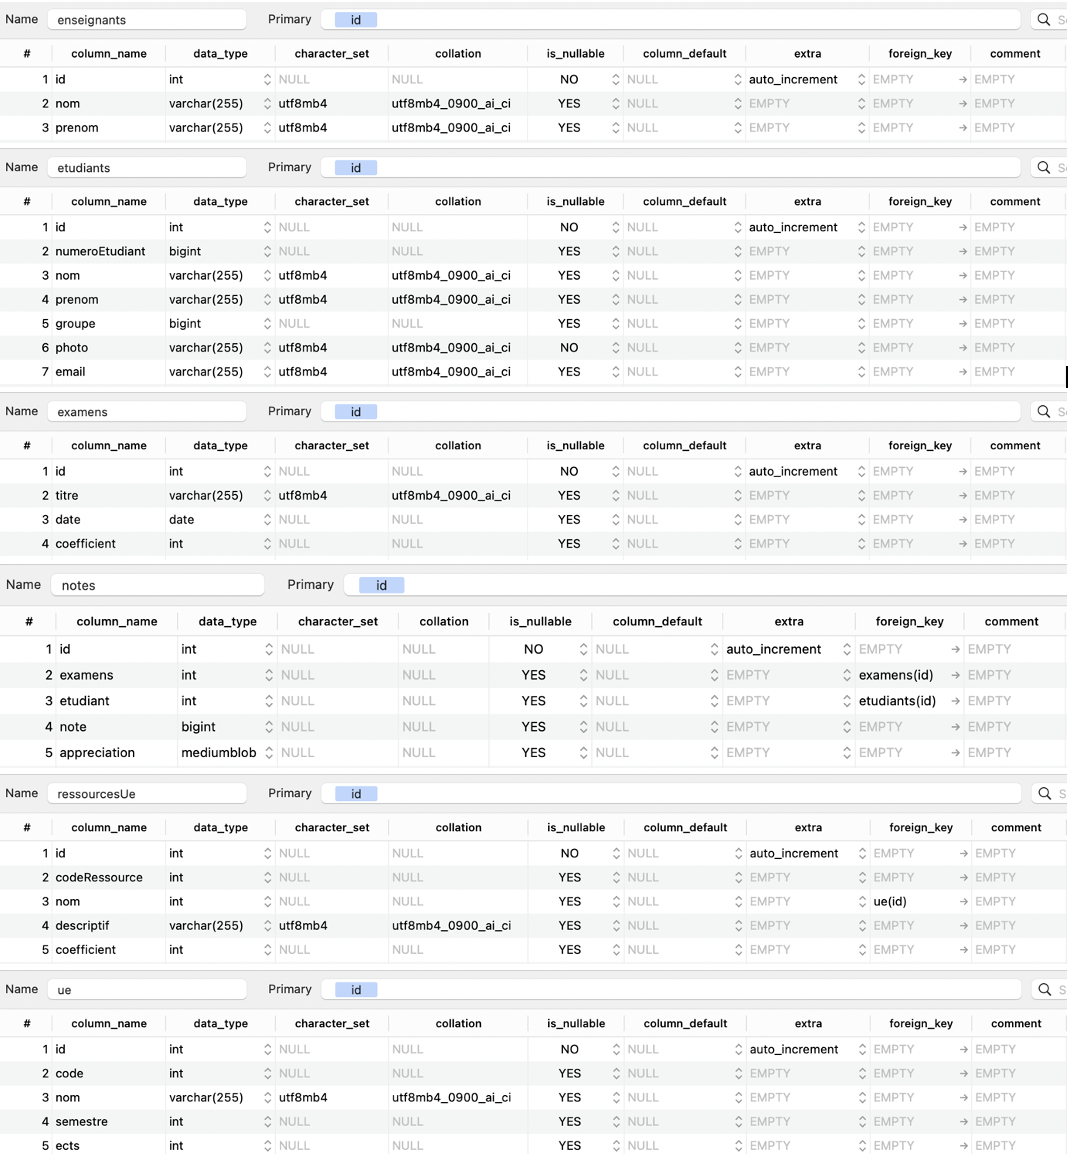
\includegraphics[scale=0.3]{img1.png}
        \captionof{figure}{Base de données}

        \newpage
        \section{Import de la base de données dans Django}
        Pour commencer, il faut donc lier notre base de données à Django, pour ce faire nous devons éditer notre fichier settings.py dans les paramètres « database » : 
        \begin{lstlisting}

            DATABASES = {
                'default': {
                    'ENGINE': 'django.db.backends.sqlite3',
                    'NAME': 'db.sqlite3',
                }
            }
            
        \end{lstlisting}
\end{document}